\chapter{Results} \label{chapter_results}

This Chapter is concerned with the presentation of results of the application of
the algorithms at a modular level and the performance of the overall integrated system.


\section{Colour Co-occurrence Histogram Detection}



\section{Mean Shift Tracking}
This section deals with the qualitative analysis of the Mean Shift Tracker
implemented in Section~\ref{implementation_mean_shift_tracker}. The analysis is
broken down into a set of experiments, each of which is based on a image
sequence that exhibits one or more of the challenges to motion tracking outlined
in Section~\ref{literature_review_challenges}. 

The image sequences used are taken from the datasets provided by the VOT2017
challenge. \cite{VOT_TPAMI}

\subsection{Experiment 1: Girl}
This sequence is that of a Girl in a park riding around on a scooter. The
relevant challenges presented in this scene are:

\begin{itemize}
    \item Occlusion (full)
    \item Scaling 
    \item Ego motion (slight) 
\end{itemize}

The relevant subsequence exhibiting these Occlusion is presented in
Figure~\ref{fig:mean_shift_occlusion}.

\begin{figure} \label{fig:mean_shift_occlusion}
    \begin{tabular}{cccc}
        \subfloat{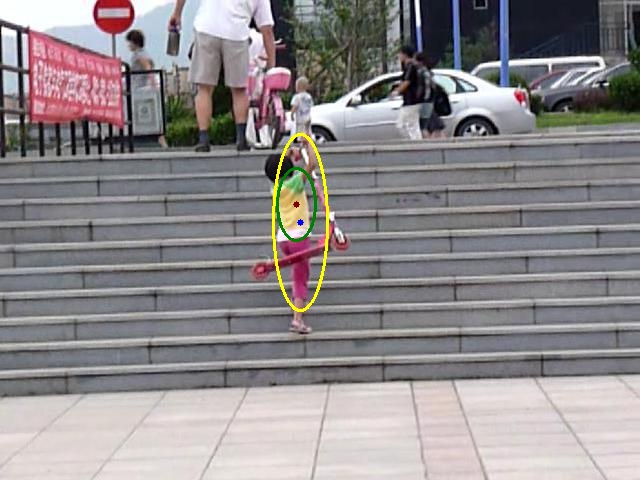
\includegraphics[width = 1.2in]{figures/results/girl/1.jpg}} &
        \subfloat{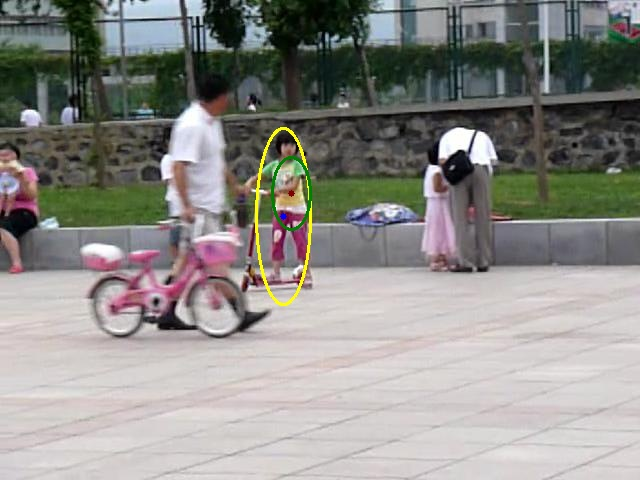
\includegraphics[width = 1.2in]{figures/results/girl/2.jpg}} &
        \subfloat{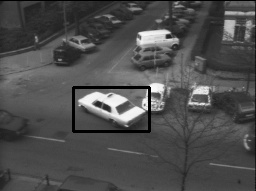
\includegraphics[width = 1.2in]{figures/results/girl/3.jpg}} &
        \subfloat{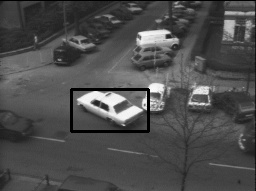
\includegraphics[width = 1.2in]{figures/results/girl/4.jpg}} \\

        \subfloat{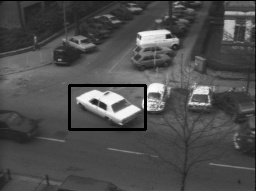
\includegraphics[width = 1.2in]{figures/results/girl/5.jpg}} &
        \subfloat{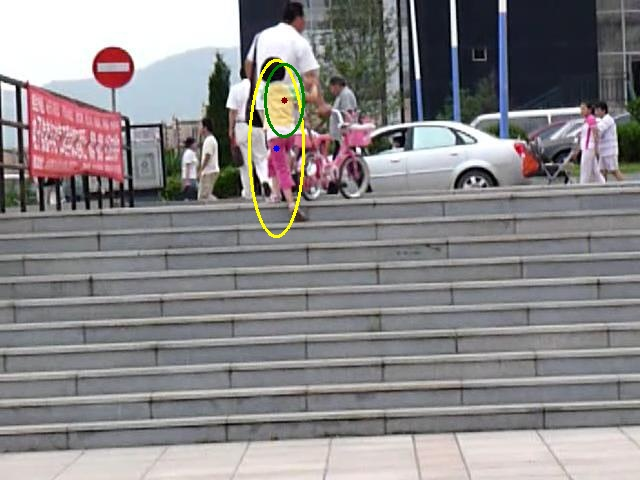
\includegraphics[width = 1.2in]{figures/results/girl/6.jpg}} &
        \subfloat{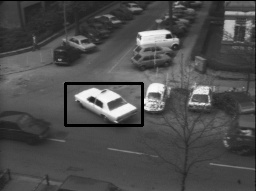
\includegraphics[width = 1.2in]{figures/results/girl/7.jpg}} &
        \subfloat{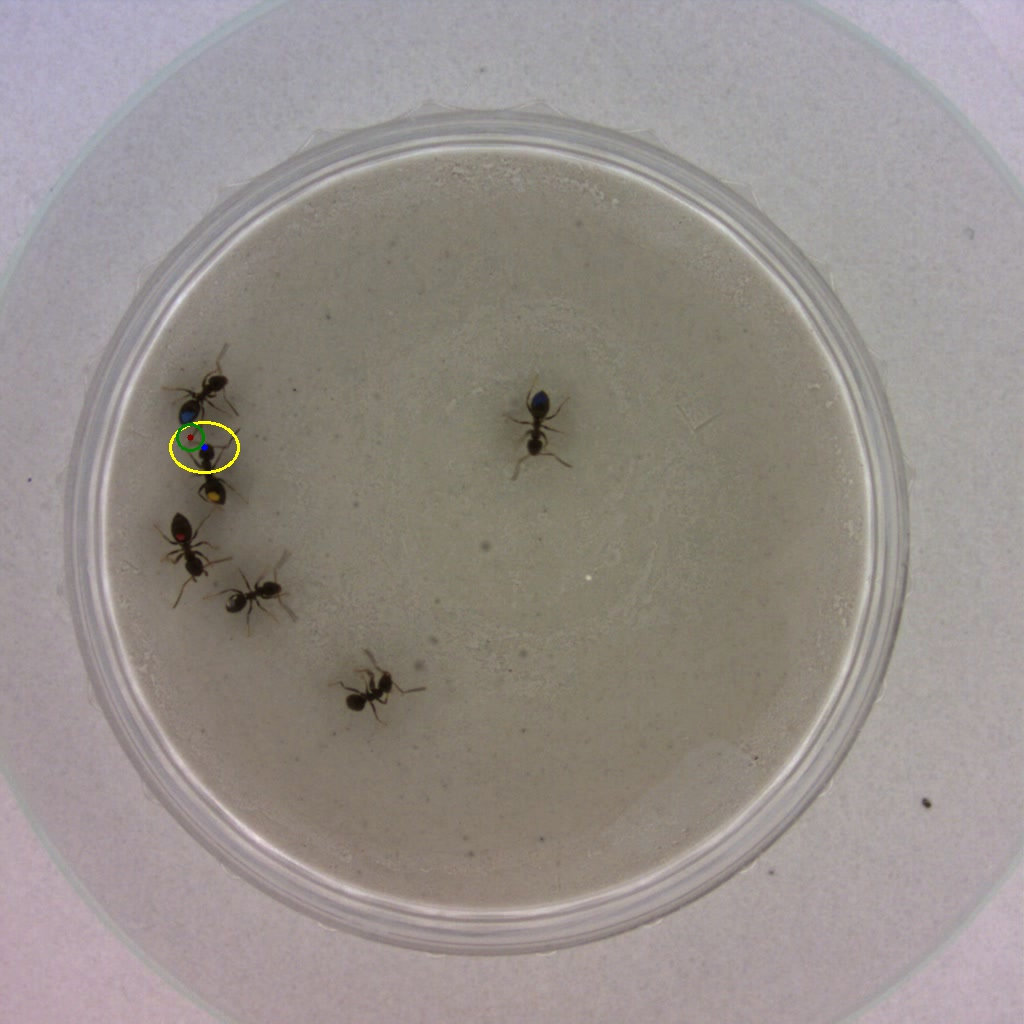
\includegraphics[width = 1.2in]{figures/results/girl/8.jpg}} \\
       
        \subfloat{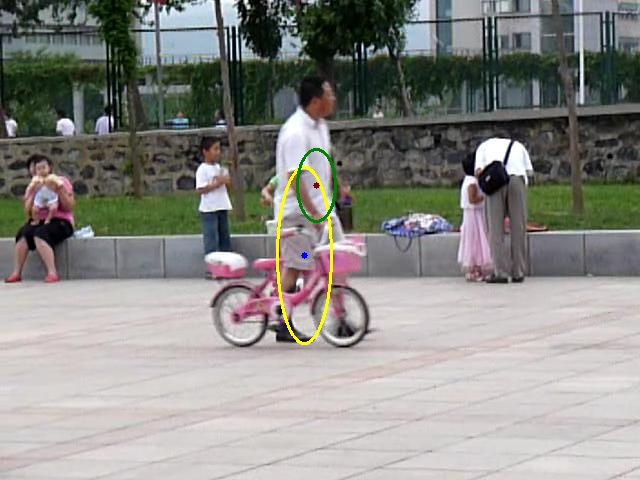
\includegraphics[width = 1.2in]{figures/results/girl/9.jpg}} &
        \subfloat{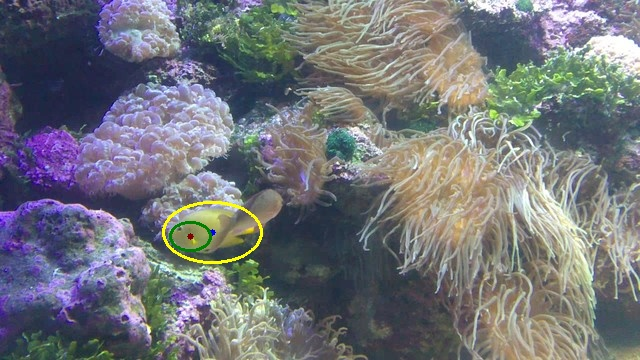
\includegraphics[width = 1.2in]{figures/results/girl/10.jpg}} &
        \subfloat{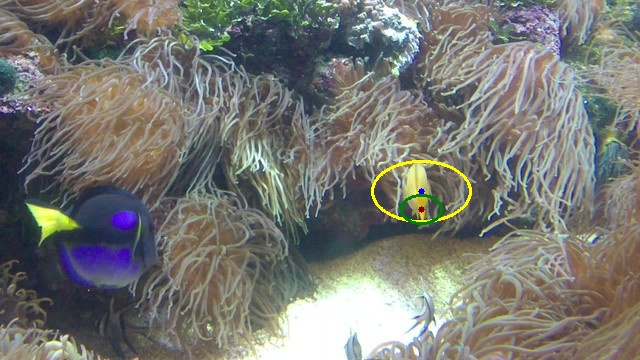
\includegraphics[width = 1.2in]{figures/results/girl/11.jpg}} &
        \subfloat{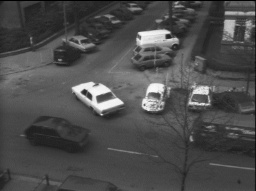
\includegraphics[width = 1.2in]{figures/results/girl/12.jpg}} \\
       
        \subfloat{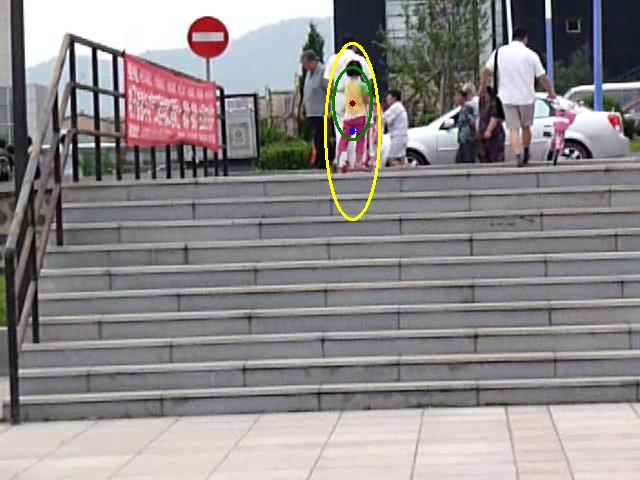
\includegraphics[width = 1.2in]{figures/results/girl/13.jpg}} &
        \subfloat{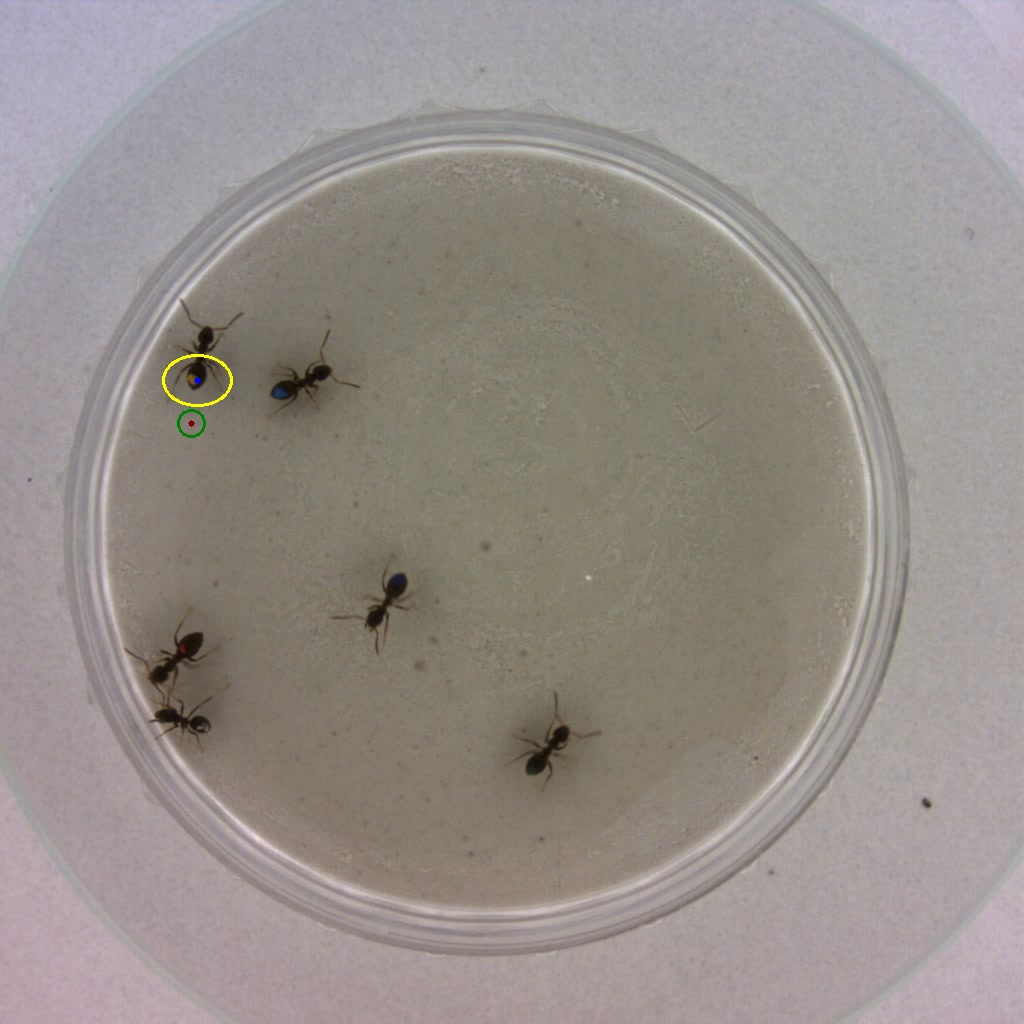
\includegraphics[width = 1.2in]{figures/results/girl/14.jpg}} &
        \subfloat{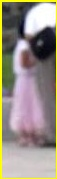
\includegraphics[width = 1.2in]{figures/results/girl/15.jpg}} &
        \subfloat{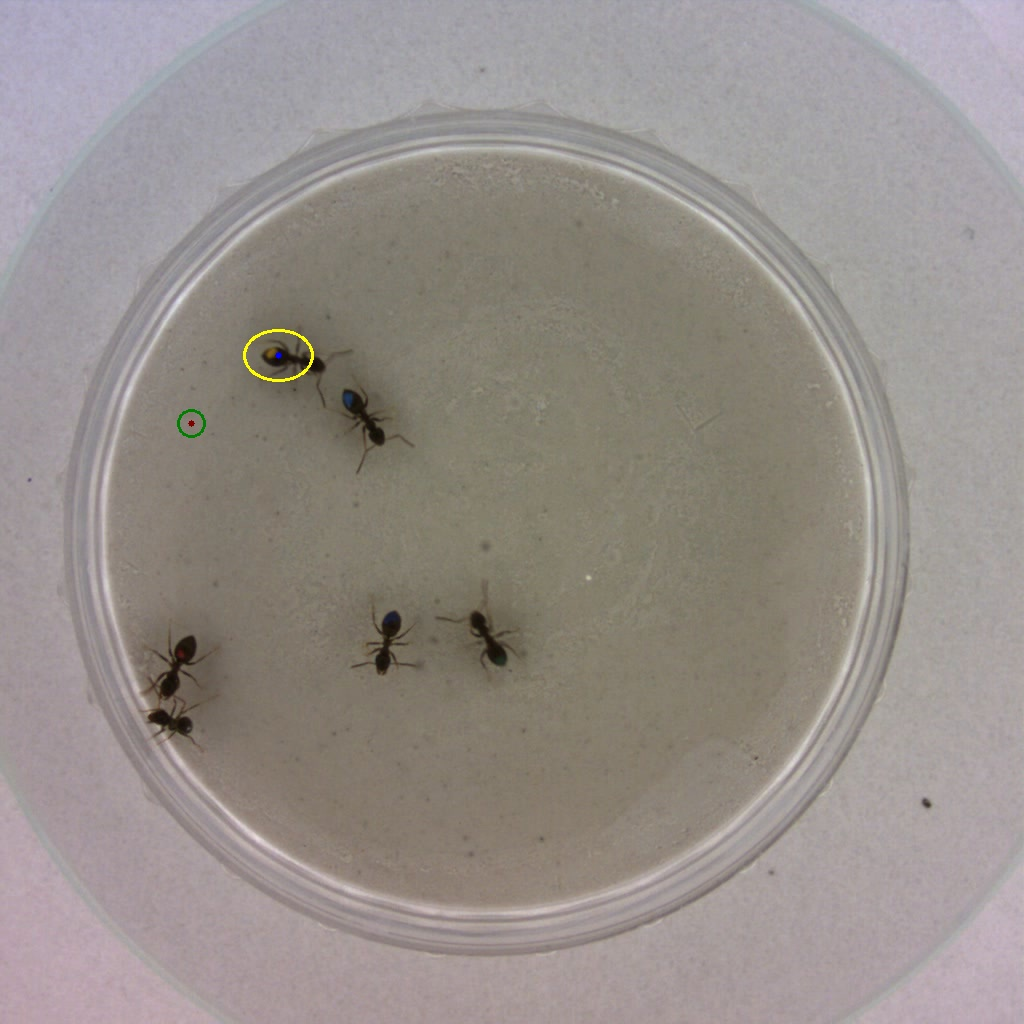
\includegraphics[width = 1.2in]{figures/results/girl/16.jpg}} \\   
    \end{tabular}
    \caption{Challenge: Occlusion in ``Girl'' sequence}
\end{figure}

\subsection{Experiment: }




